\documentclass[conference]{IEEEtran}
\IEEEoverridecommandlockouts
% The preceding line is only needed to identify funding in the first footnote. If that is unneeded, please comment it out.
\usepackage{cite}
\usepackage{amsmath,amssymb,amsfonts}
\usepackage{algorithmic}
\usepackage{graphicx}
\usepackage{textcomp}
\usepackage{xcolor}
\def\BibTeX{{\rm B\kern-.05em{\sc i\kern-.025em b}\kern-.08em
    T\kern-.1667em\lower.7ex\hbox{E}\kern-.125emX}}
\begin{document}

\title{KUKA LBR iiwa --- Adaptive Assembly Analysis}

\author{\IEEEauthorblockN{Arjan Gupta}
\IEEEauthorblockA{\textit{Robotics Engineering} \\
\textit{Worcester Polytechnic Institute}\\
Worcester, MA, USA \\
agupta11@wpi.edu}
}

\maketitle

\begin{abstract}
This paper presents an analysis of the KUKA LBR iiwa robot's
ability to perform rigid-body assembly tasks. The analysis is based on the first YouTube
video presented in the prompt of the final exam. The video shows the robot's ability
to adapt to the environment and perform manufacturing assembly tasks.
\end{abstract}

\begin{IEEEkeywords}
KUKA, LBR iiwa, assembly, analysis
\end{IEEEkeywords}

\section{Introduction}
The KUKA LBR iiwa robot is a 7-axis robot that is capable of performing 
rigid-body assembly tasks, as shown in the YouTube video~\cite{youtube_2014}. As per the data sheet
of the robot, it is capable of performing assembly tasks with a payload of 7--14 kg,
depending on the model.
Its maximum reach is 800--820 mm depending on the model.

\begin{figure}[h!]
\centering
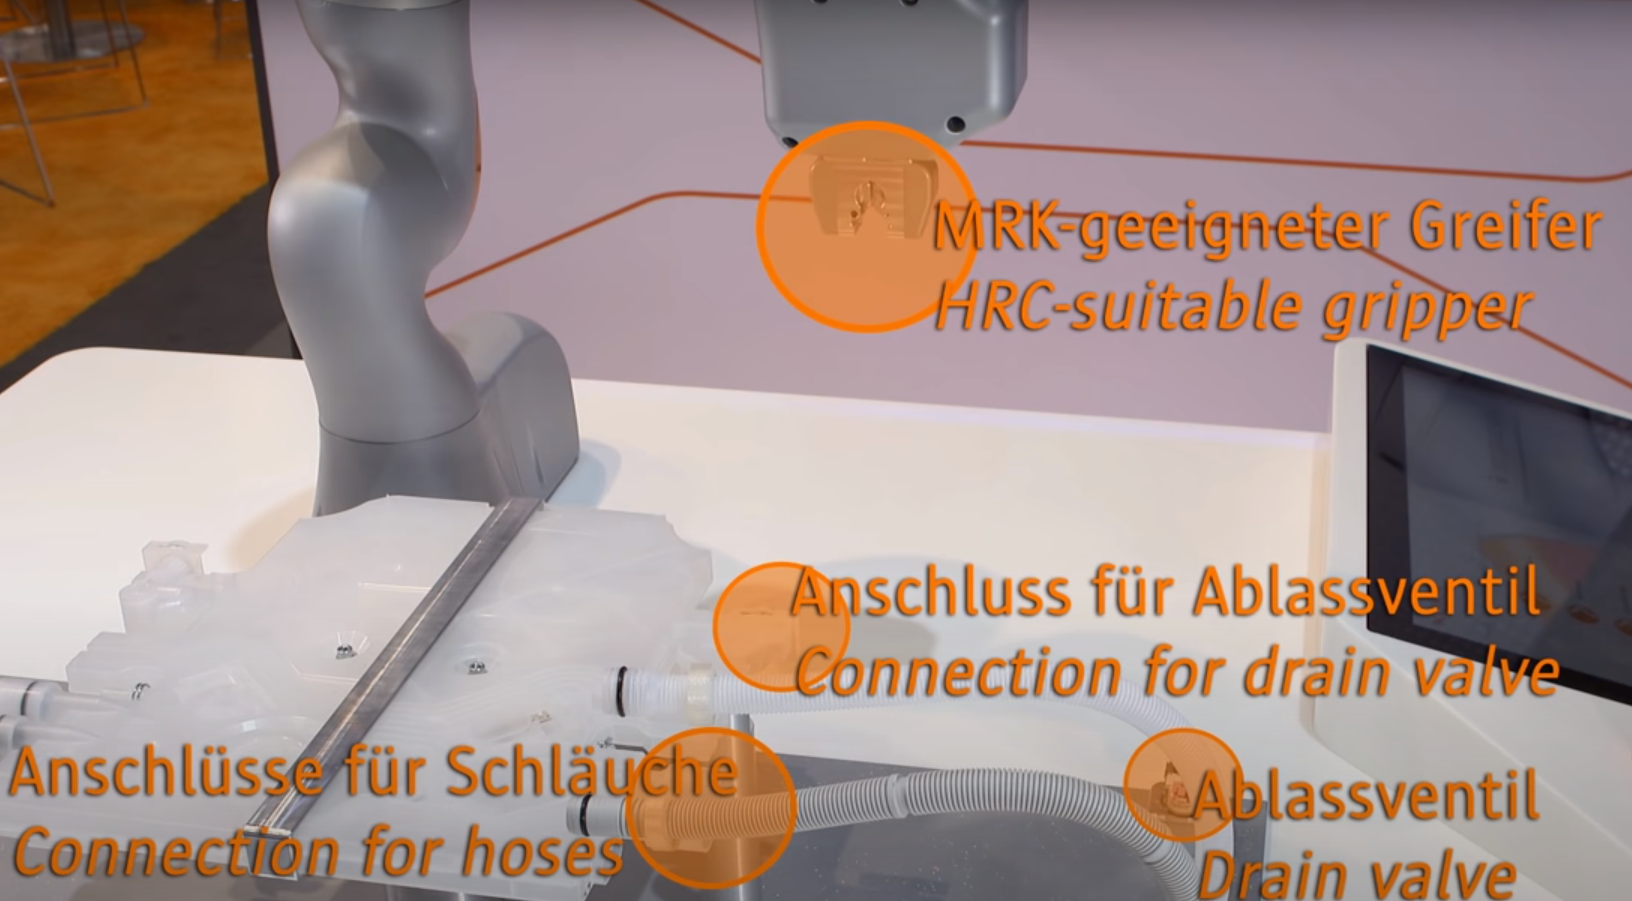
\includegraphics[scale=0.15]{kuka-setup-desc.png}
\caption{KUKA LBR iiwa in its workspace from the video}
\label{kuka-setup-desc}
\end{figure}

In the video, the robot is first shown in its workspace, showing a HRC-suitable
gripper. A drain valve, a connector for the drain valve, and a connection for
the hoses are shown. A still from the video is shown in Figure~\ref{kuka-setup-desc}.

After the setup is shown, the robot is shown performing the assembly tasks. The first
part shows the utilization of the joint torque sensors for process recognition. The second
part of the video shows the usage of the joint torque sensors for force-controlled
joining processes. The third part of the video shows the safety features of the robot.

Our objective in this paper is to analyze the robot kinematics and dynamics being
used in each of the three parts of the video. We will also describe how one would
simulate the tasks being performed by the robot in MATLAB, using the Robotics
ToolBox.

\section{Materials and Methods}

\subsection{Analysis of first part}



\bibliography{refs.bib}
\bibliographystyle{IEEEtran}

\end{document}
